\documentclass{usireport}

%% VARIABLES
\newcommand\namesurname{Alessandro Gobbetti}
\newcommand\assignment{Assignment 2}
\newcommand\assignmenttitle{}

\newcommand\subject{Mobile and Wearable Computing}

\begin{document}
\maketitlepage

\section{Introduction}
This is the second assignment for the Mobile and Wearable Computing course. The code is available at: \\\url{https://github.com/Alessandro-Gobbetti/Mobile-and-Wearable-Computing/Assignment2}.

\section{Exercise 1: Android Basics}

\textbf{Question 1:} What does the \mintinline{xml}{android:minSdkVersion} in android project indicate?

\textbf{Answer:} Android applications should declare the API level they are targeting (\mintinline{xml}{android:minSdkVersion} and \mintinline{xml}{android:targetSdkVersion}). 
The \mintinline{xml}{android:minSdkVersion} attribute indicates the minimum API level required for the application to run. Lowering the \mintinline{xml}{minSdkVersion} allows the app to run on older devices, but it also limits the features that can be used. 
The \mintinline{xml}{android:targetSdkVersion} attribute indicates the highest API level that the app has been tested on. This allows the app to take advantage of new features and optimizations in newer versions of Android.

If a device's API level is below the \mintinline{xml}{minSdkVersion}, the app will not be installed. On the other hand, if the device's API level is above the \mintinline{xml}{targetSdkVersion}, the app will still run, but it may not take advantage of the latest features and optimizations.

\textbf{Question 2:} Why Android documentation indicates that declaring the attribute \mintinline{xml}{android:maxSdkVersion} is not recommended?

\textbf{Answer:} The \mintinline{xml}{android:maxSdkVersion} indicates the maximum API level that the app can run on. However, the Android documentation recommends against using this attribute because it can lead to compatibility issues. If the \mintinline{xml}{maxSdkVersion} is set to a specific API level, the app will not be available on devices with a higher API level. This can prevent users from installing the app on newer devices, even if the app is fully compatible with the newer API level. By design, newer versions of Android are backward compatible, so apps should be able to run on newer devices without issues.
Additionally, in some cases, declaring the \mintinline{xml}{maxSdkVersion} attribute can result in the app being removed from users' devices after system updates to a higher API level. This can lead to a poor user experience and loss of data.

\textbf{Question 3:} What are the two types of Navigation Drawer? Explain the differences between the two types?

\textbf{Answer:} Navigation drawers provide access to destinations and app functionality. There are two types of navigation drawers: the standard drawer and the modal drawer.

The standard drawer is a panel that shares the screen with the main content. It allows users to simultaneously access drawer destinations and app content. The standard drawer can be permanently visible or opened and closed by tapping a navigation menu icon. It is often used on tablets and desktops where there is more screen space.

The modal drawer is more common on mobile devices where screen space is limited. The modal drawer slides in from the edge of the screen and overlays the main content, blocking interaction with the content until the drawer is closed.

\begin{figure}[H]
    \centering
    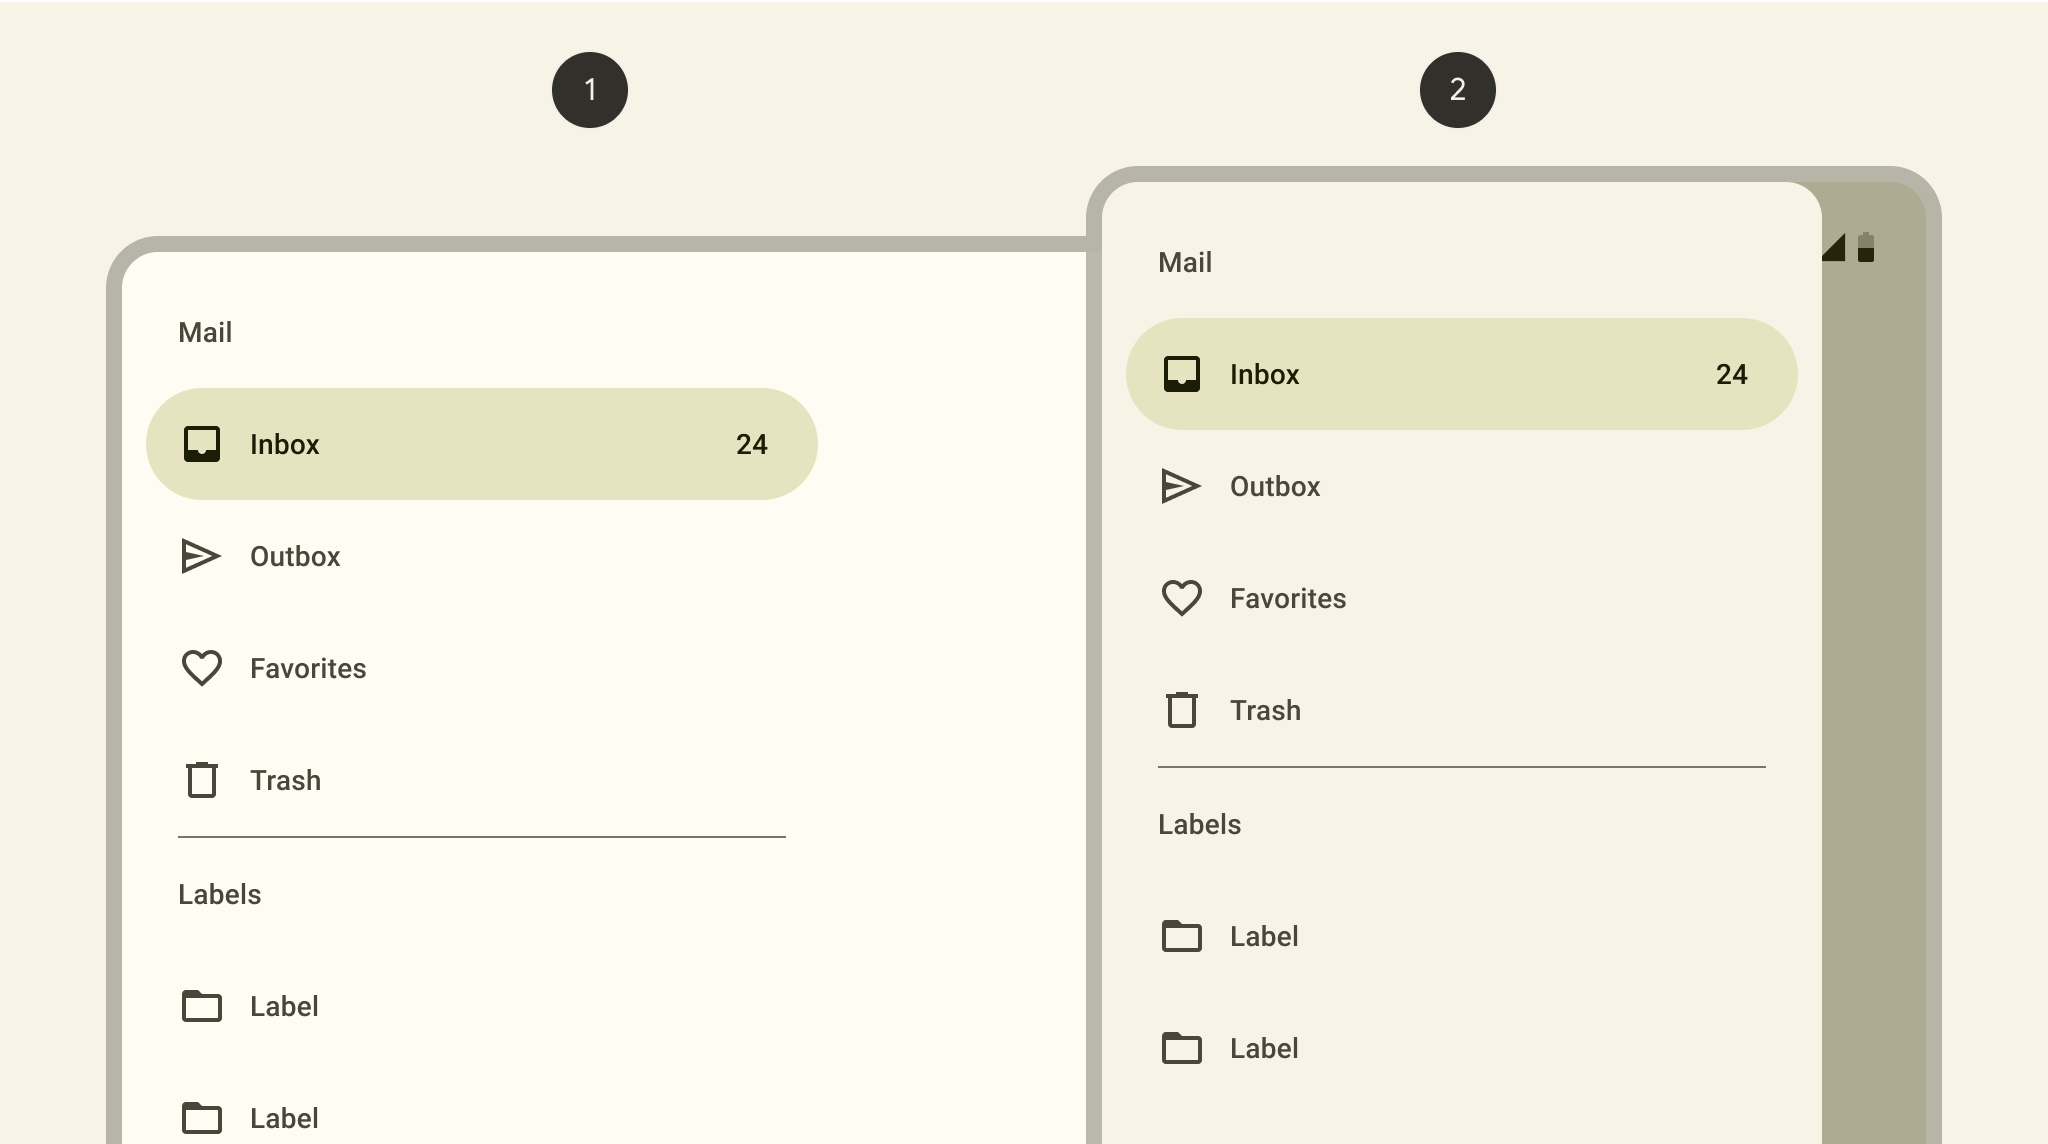
\includegraphics[trim={0 10cm 0 5cm},clip,width=0.8\textwidth]{fig/drawers.png}
    \caption{Standard [Left] and Modal [Right] Navigation Drawers}
    \label{fig:nav_drawer}
\end{figure}


\section{Exercise 2: Material Design}

\textbf{Task 1:} Change the icon of the app. Choose/create a representative icon for your StepAppV4. Set the default Android icon to the icon you chose/created.

A new icon was created for the StepAppV4 application. The icon was downloaded from \href{https://www.svgrepo.com/svg/35735/feet-footprint}{SVGRepo} and used as the foreground, with the background consisting of a solid color that matches the application's main theme.

\begin{figure}[H]
    \centering
    \begin{subfigure}[b]{0.2\textwidth}
        
\includegraphics[width=\textwidth]{fig/ic_launcher.png}
    \end{subfigure}
    \hspace{2cm}
    \begin{subfigure}[b]{0.2\textwidth}
        
\includegraphics[width=\textwidth]{fig/ic_launcher_round.png}
    \end{subfigure}
    \caption{App Icon}
    \label{fig:app_icon}
\end{figure}

\textbf{Task 2:} Implement the dark theme for the layout of your StepAppV4 app.

As done during the tutorial for the light theme, the dark theme was implemented. The new colors and themes (renamed to start with \texttt{dark\_md\_theme}) were created and added to the \mintinline{xml}{colors.xml} and \mintinline{xml}{themes.xml} files. 

\begin{figure}[H]
    \centering
    \begin{subfigure}[b]{0.3\textwidth}
        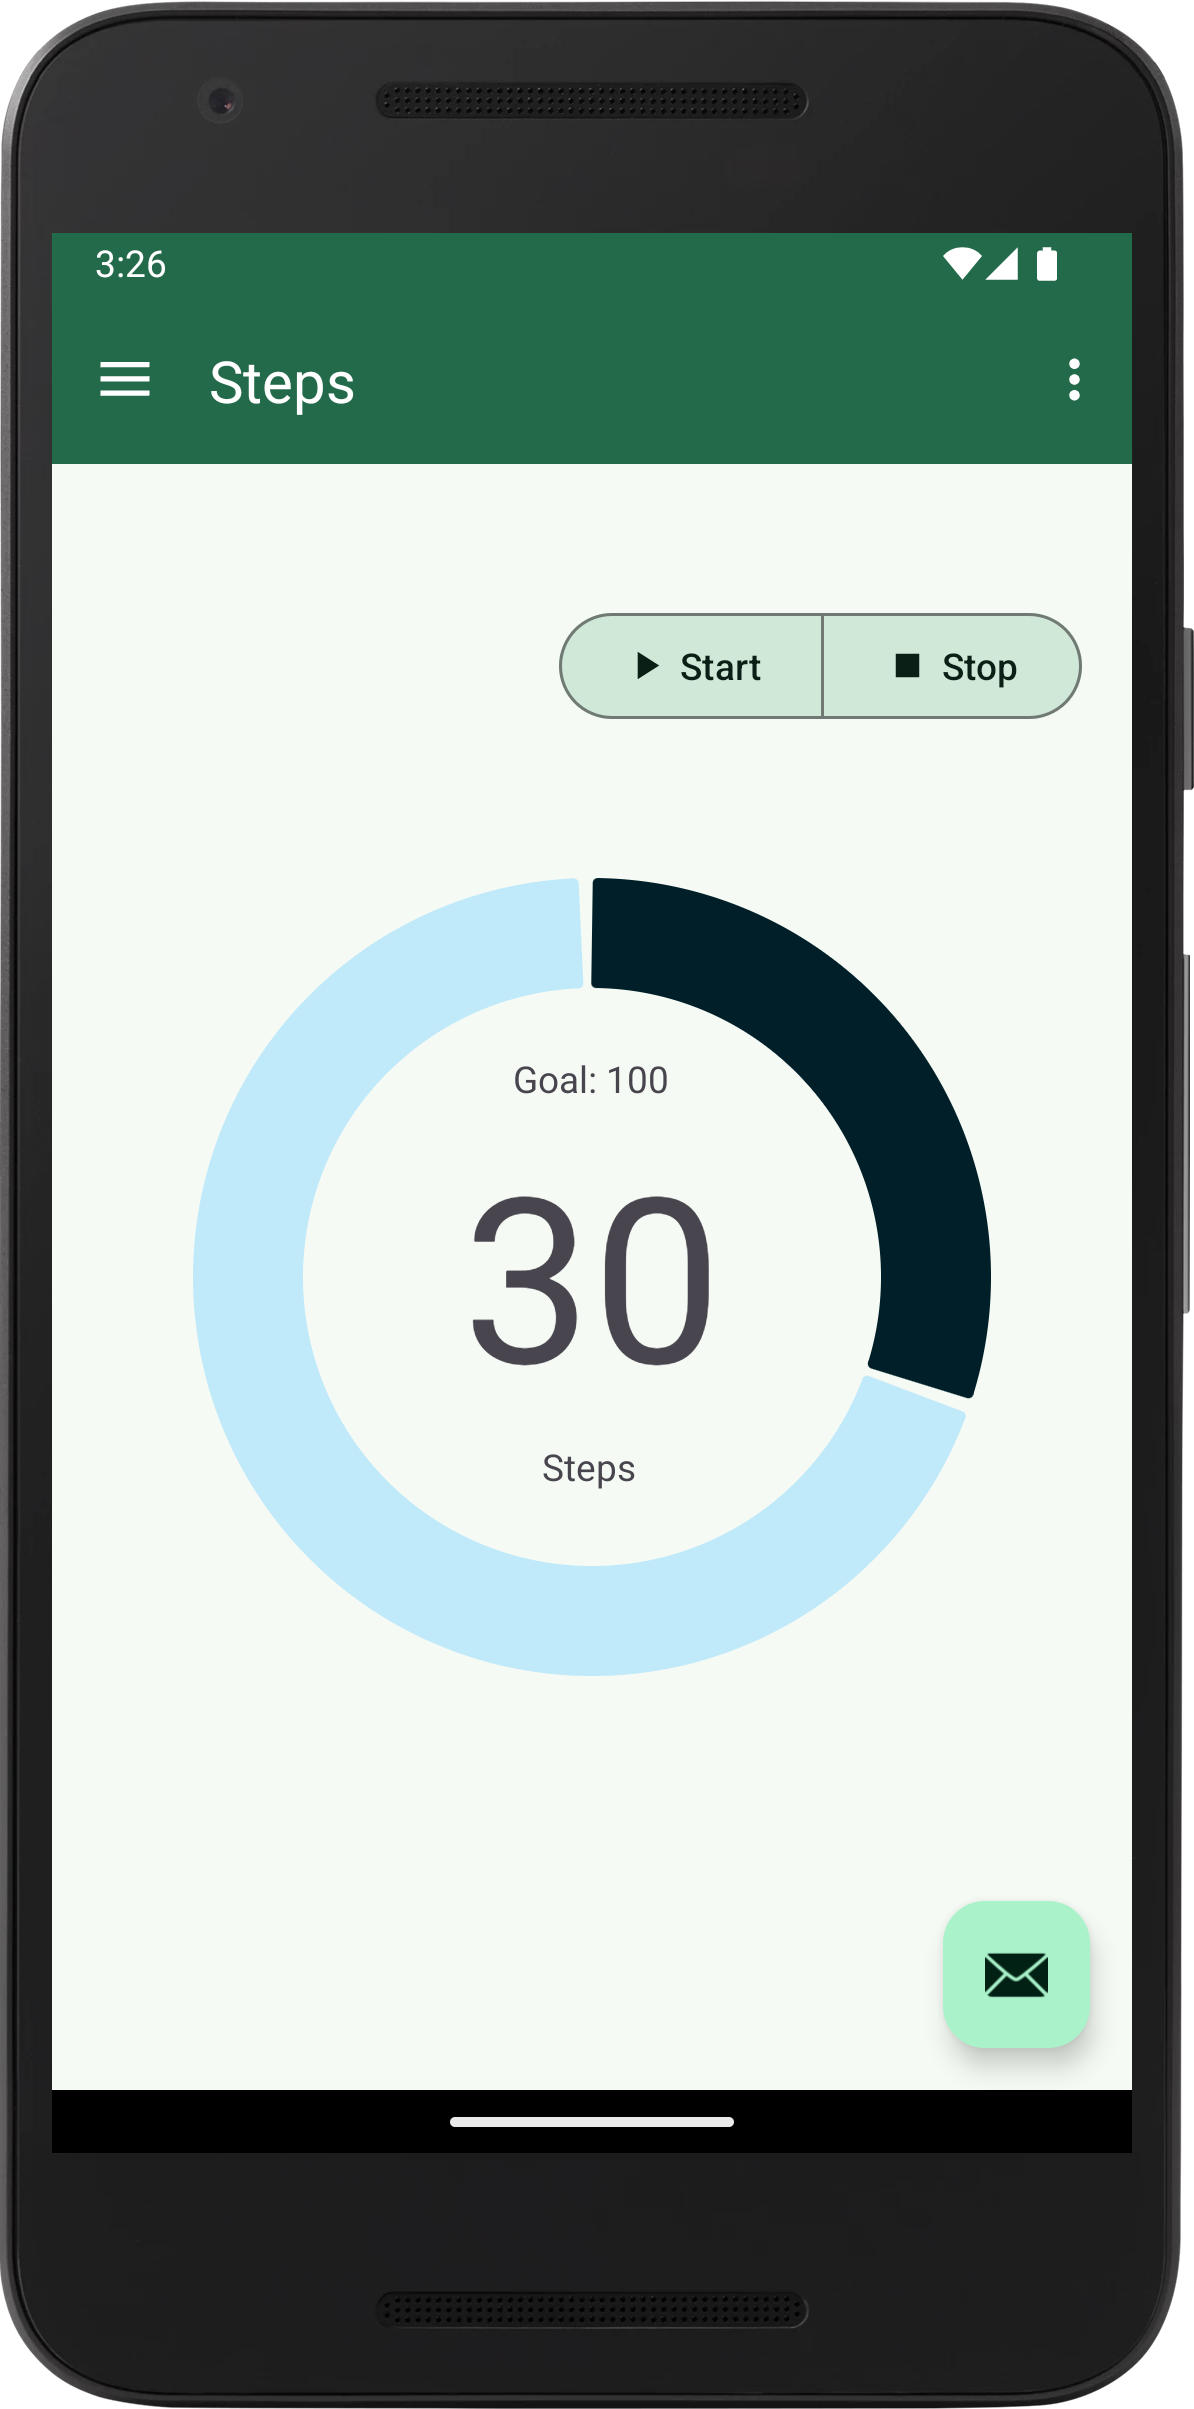
\includegraphics[width=\textwidth]{fig/light_mode.png}
        \caption{Light Theme}
    \end{subfigure}
    \hspace{2cm}
    \begin{subfigure}[b]{0.3\textwidth}
        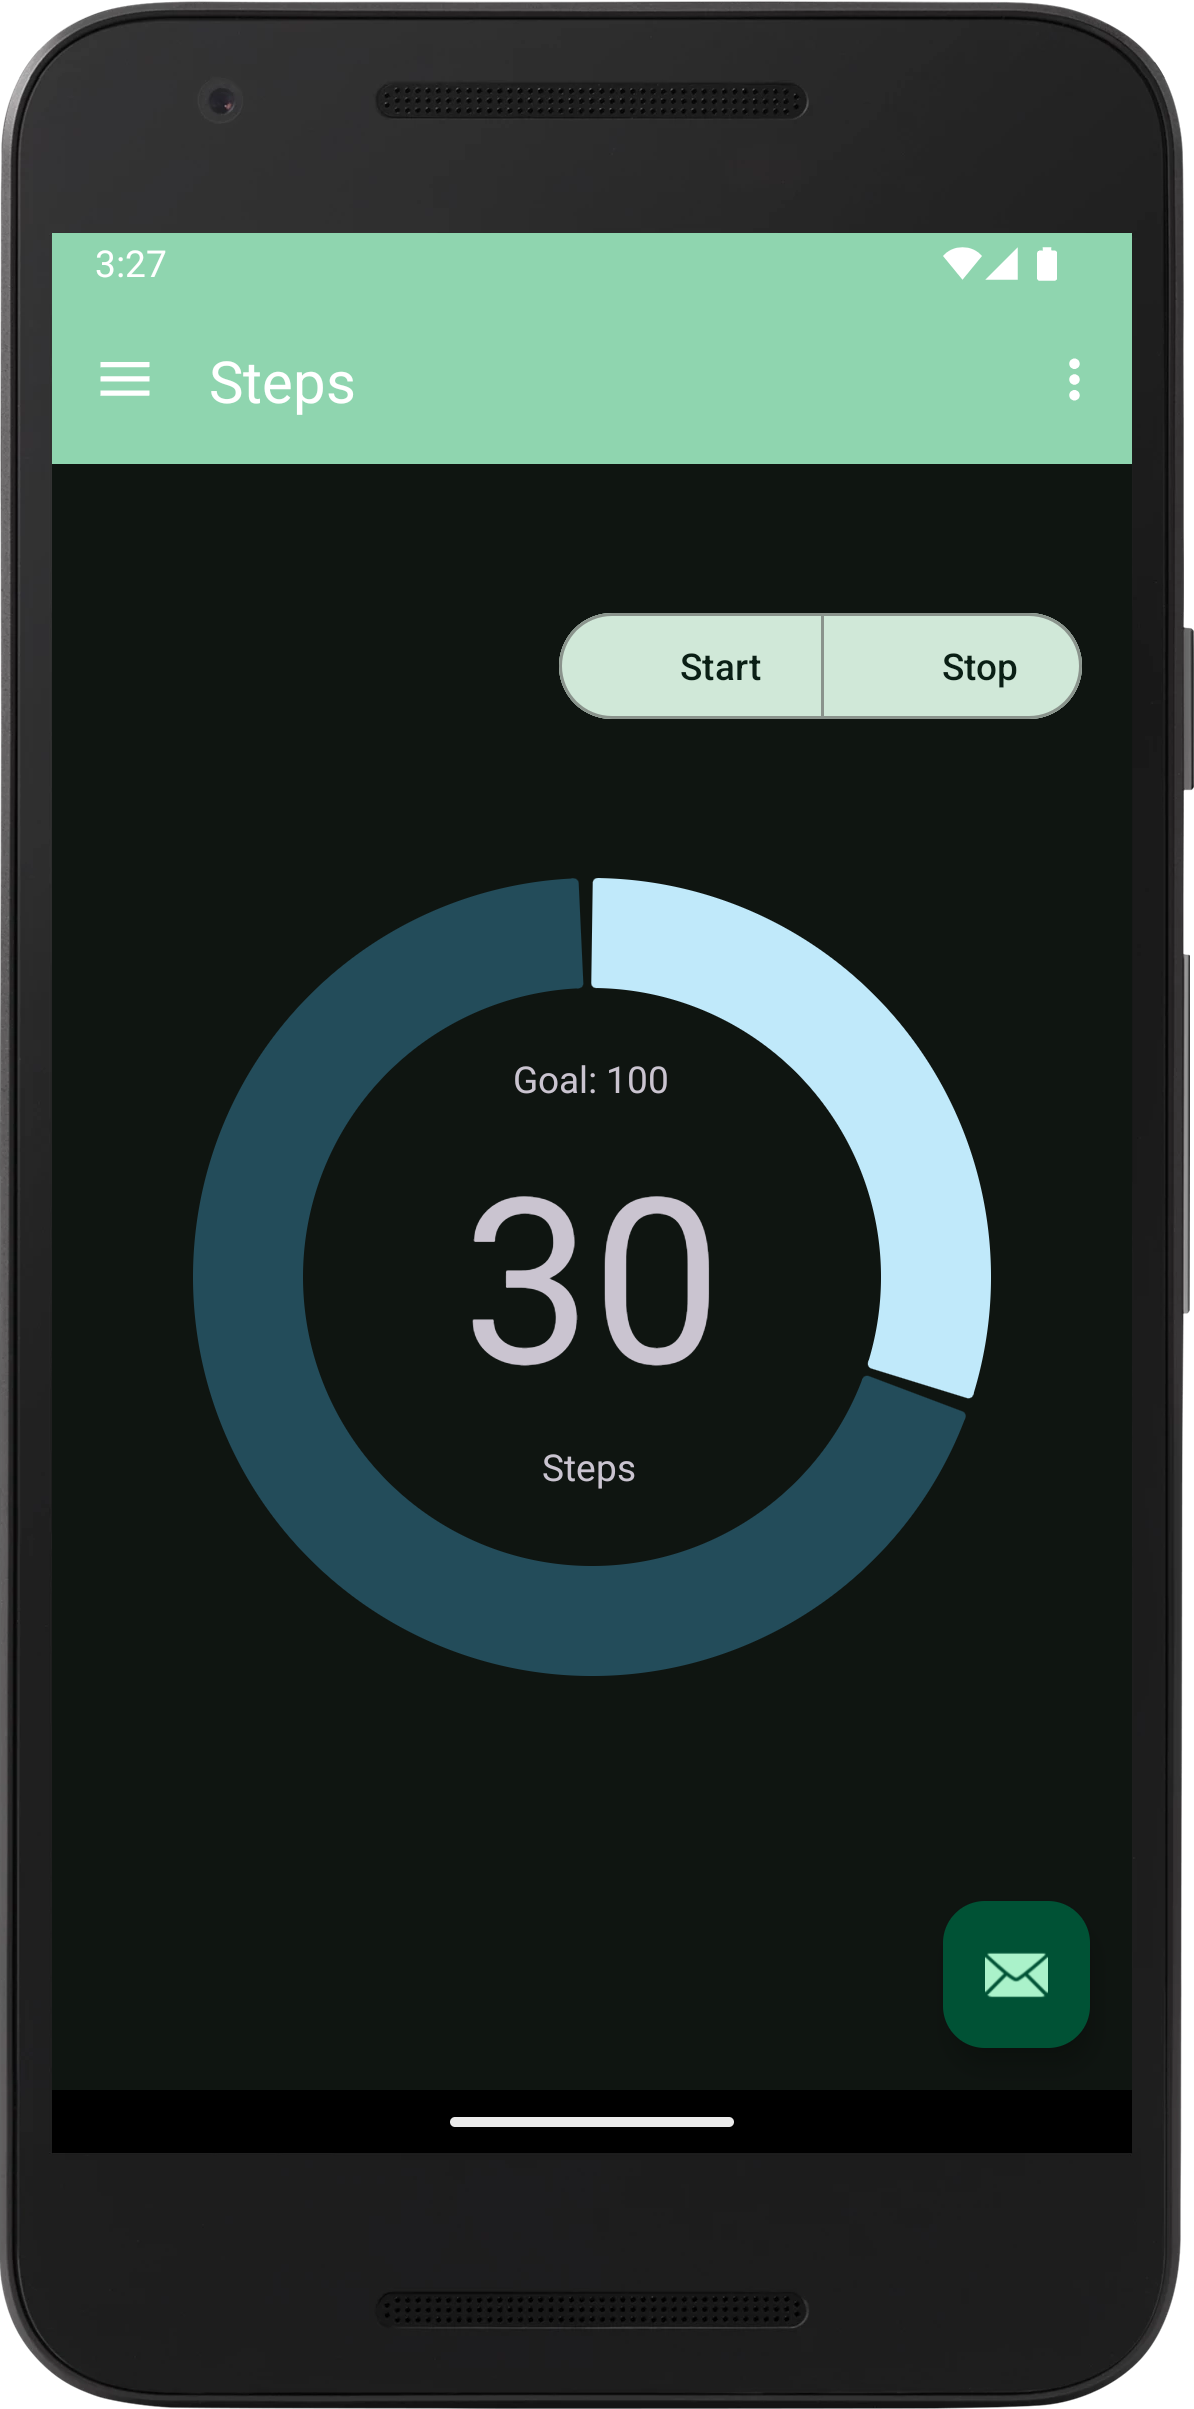
\includegraphics[width=\textwidth]{fig/dark_mode.png}
        \caption{Dark Theme}
    \end{subfigure}
    \caption{Light and Dark Themes}
    \label{fig:themes}
\end{figure}

\newpage
\section{Exercise 3: Step Counter}

The main goal of this exercise is to use the Android \texttt{STEP\_DETECTOR} sensor is used to detect steps.
To do this, in the \mintinline{java}{onSensorChanged()} method of the \mintinline{java}{class StepCounterListener} we need to handle the case when the sensor type is \mintinline{java}{Sensor.TYPE_STEP_DETECTOR}. The \texttt{STEP\_DETECTOR} is triggered every time a step is detected. So we just have to store the newly detected step in the database. 

\begin{minted}{java}
public class StepCounterListener implements SensorEventListener {
    ...
    @Override
    public void onSensorChanged(SensorEvent sensorEvent) {
        switch (sensorEvent.sensor.getType())
        {
            case Sensor.TYPE_LINEAR_ACCELERATION:
                ...
                break;
            case Sensor.TYPE_STEP_DETECTOR:
                countSteps(sensorEvent.values[0]);
                break;
        }
    }
    ...

    private void countSteps(float step)
    {   
        // increment the step counter
        stepDetectorStepCounter += 1;
        // Log the number of steps detected by the step detector
        Log.d("STEP DETECTOR STEPS: ", String.valueOf(stepDetectorStepCounter));
        // Save the number of steps
        saveStepInDatabase();
        // Update the TextView and the progress bar
        stepCountsView.setText(String.valueOf(stepDetectorStepCounter));
        progressBar.setProgress(stepDetectorStepCounter);

    }
    ...
}
\end{minted}

The \mintinline{java}{countSteps()} method is used to increment the class variable \mintinline{java}{stepDetectorStepCounter}, save the step in the database, update the TextView and the progress bar with the new values only detected by the \texttt{STEP\_DETECTOR} sensor.

Finally, when the app page is created, the number of steps is retrieved from the database and displayed in the TextView and the progress bar. In the \mintinline{java}{onCreateView()} method of the \mintinline{java}{class StepsFragment} the progress bar and the TextView are immediately updated with the number of steps stored in the database.

\begin{minted}{java}
public class StepsFragment extends Fragment {
    public View onCreateView(@NonNull LayoutInflater inflater,
                             ViewGroup container, Bundle savedInstanceState) {
        ...

        // Load the steps counter from the database
        //Timestamp
        long timeInMillis = System.currentTimeMillis();
        // Convert the timestamp to date
        SimpleDateFormat jdf = new SimpleDateFormat("yyyy-MM-dd HH:mm:ss:SSS");
        jdf.setTimeZone(TimeZone.getTimeZone("GMT+2"));
        final String dateTimestamp = jdf.format(timeInMillis);
        String currentDay = dateTimestamp.substring(0,10);
        stepsCounter = StepAppOpenHelper.loadSingleRecord(getContext(), currentDay);
        
        ...

        // Set the progress bar
        CircularProgressIndicator progressBar = 
                (CircularProgressIndicator) root.findViewById(R.id.progressBar);
        progressBar.setMax(100);
        progressBar.setProgress(stepsCounter);

        // Set the steps counter
        stepsTextView = (TextView) root.findViewById(R.id.stepsCount_textview);
        stepsTextView.setText(""+stepsCounter);
        ...
    }
}
\end{minted}

\end{document}
